The last topic I want to focus on in this essay is the effect of entropy on the growth of entanglement between subsystems. Let us select a subsystem $\Omega_1$ in the system $\Omega = \Omega_1 \cup \Omega_2$. The entropy of the subsystem can be found through the reduced density matrix $\rho_{\Omega_1} = \tr_{\Omega_2} \rho$
\begin{equation*}
     S(\rho_{\Omega_1}) = - \tr \rho_{\Omega_1} \ln \rho_{\Omega_1},
\end{equation*}
one shows that bipartite entanglement exists between two disjoint subsystems $\Omega_1$ and $\Omega_2$ of $\Omega$ with reduced density matrices $\rho_{\Omega_1}$ and $\rho_{\Omega_2}$ if
\begin{equation*}
     S(\rho_{\Omega_1}) > S(\rho_{\Omega_1 \cup \Omega_2})
     \hspace{10 mm} \text{or} \hspace{10 mm}
     S(\rho_{\Omega_2}) > S(\rho_{\Omega_1 \cup \Omega_2}).
\end{equation*}
However, further we will simply monitor the growth of the entropy of the subsystem, which in general most likely indicates the entanglement of the subsystems. We will also work with one-dimensional chain hard-bosons described by the Hamiltonian \eqref{9:model}. Let us divide the system into two parts: left and right; as the initial state we will consider half population at even nodes (fig. \ref{fig:Sg}).  The growth of entropy in LP is considered. It can be seen that the addition of a weak interaction leads to a statistically significant increase in entropy. In my opinion, this is a rather non-obvious result, since the interaction is a small diagonal addition to the Hamiltonian, which already has random numbers on the diagonals.



\begin{figure}[h]
    \centering
    \addletter{50}{a} \hspace{2 mm} 
    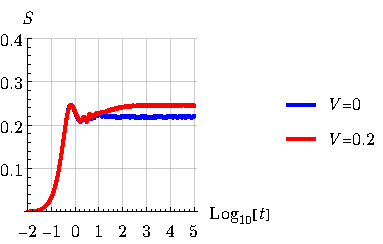
\includegraphics[align=c]{imgs/S_FV1.pdf}
    \hspace{10 mm} 
    \addletter{50}{b} \hspace{2 mm} 
    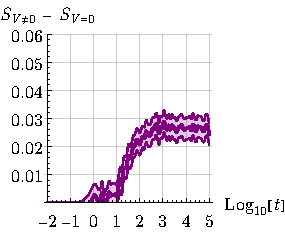
\includegraphics[align=c]{imgs/S_FV2.pdf}
    \caption{a) Entanglement growth. b) The same data but with subtracted values.}
    \label{fig:Sg}
\end{figure}


Similar results were obtained in \cite{bardarson_unbounded_2012}. As in \cite{schreiber_observation_2015} (fig. \ref{fig:1daddb}a), a logarithmic increase in entropy is observed (fig. \ref{fig:Sga}a). Since the calculations in the article were carried out through ED, rather small systems were considered, which led to the constant $S$ (fig. \ref{fig:Sga}b), however, an obvious trend can be traced as the size of the system increases.



Thus, at least from the point of view of entanglement and entropy of subsystems, MBL is fundamentally different from AL. The entanglement increases slowly until a saturation time scale, which diverges in the infinite system. 



\begin{figure}[h]
    \centering
    \addletter{150}{a} 
    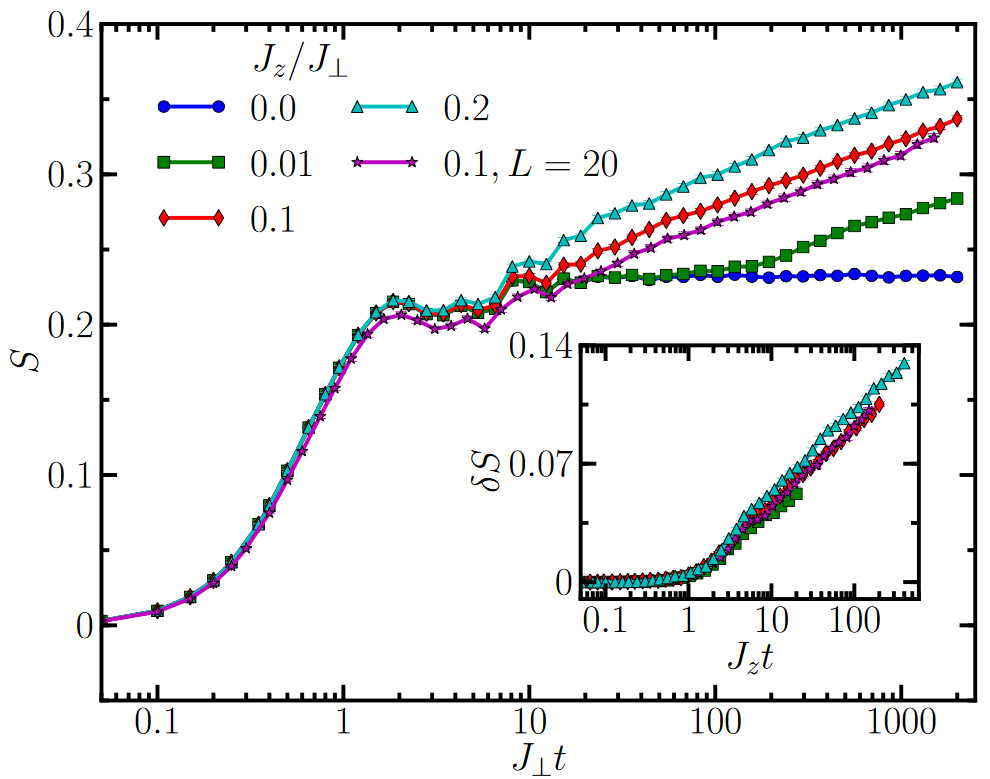
\includegraphics[width=0.4\textwidth]{imgs/S_FV_12a.png}
    \hspace{10 mm} 
    \addletter{150}{b} 
    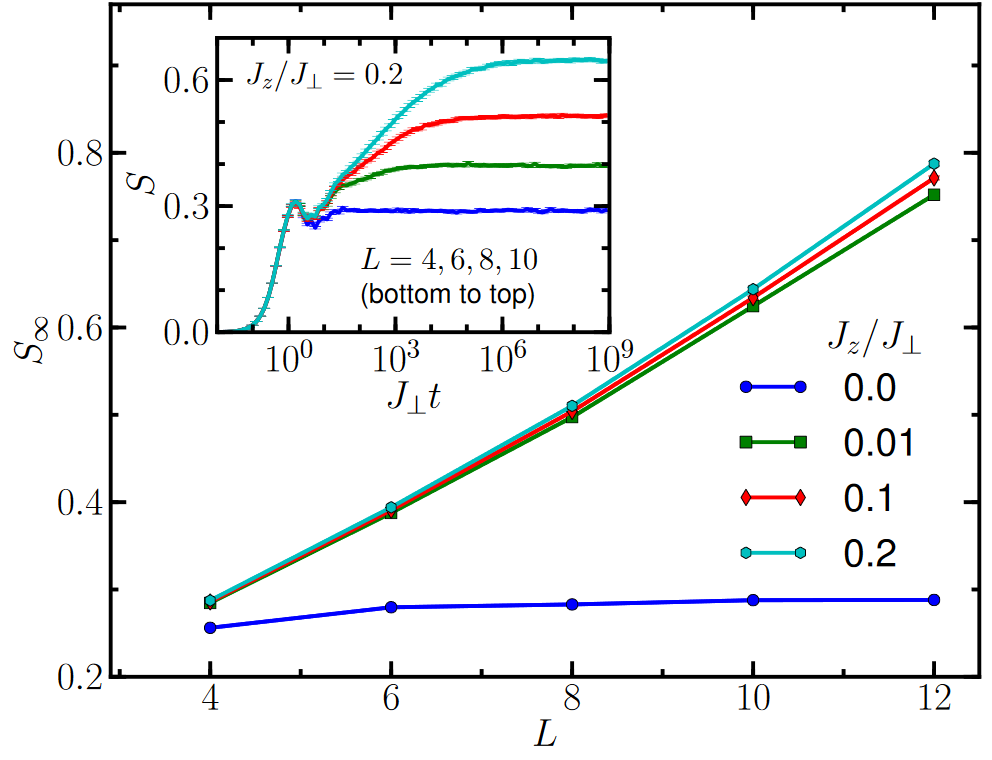
\includegraphics[width=0.4\textwidth]{imgs/S_FV_12b.png}
    \caption{
    \cite{bardarson_unbounded_2012}
        a) Entanglement growth.
        b) Saturation values of the entanglement entropy as a function of $L$.
    }
    \label{fig:Sga}
\end{figure}
